\documentclass[tikz,border=10pt]{standalone}
\usepackage{amsmath,amssymb}
\usetikzlibrary{arrows.meta,positioning,fit,backgrounds}
\begin{document}
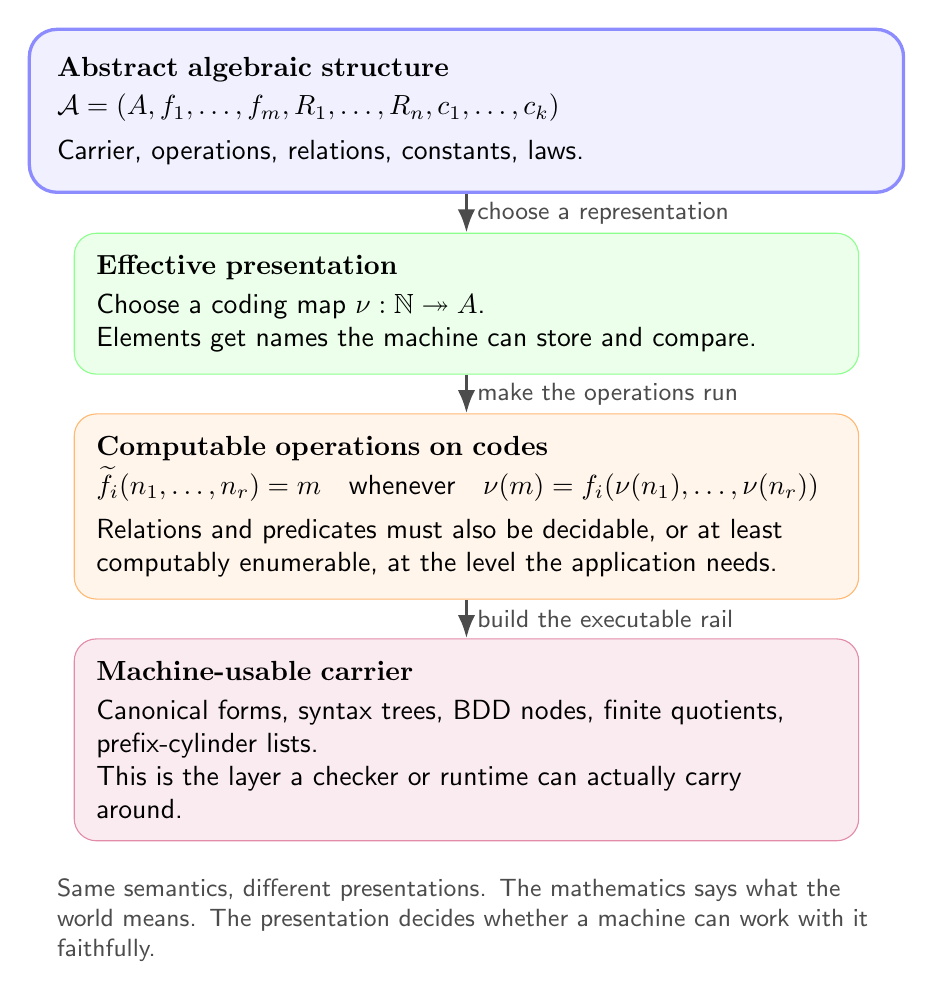
\begin{tikzpicture}[
  font=\sffamily,
  >=Latex,
  box/.style={draw, rounded corners=10pt, very thick, align=left, inner sep=10pt, text width=10.4cm, fill=white},
  soft/.style={draw, rounded corners=8pt, align=left, inner sep=8pt, text width=9.4cm, fill=gray!6},
  arr/.style={->, very thick, color=black!70},
  note/.style={font=\sffamily\small, align=left, text=black!70}
]

\node[box, fill=blue!6, draw=blue!45] (abs) {
{\bf Abstract algebraic structure}\\[2pt]
$\mathcal{A} = (A, f_1, \ldots, f_m, R_1, \ldots, R_n, c_1, \ldots, c_k)$\\[4pt]
Carrier, operations, relations, constants, laws.
};

\node[soft, below=14pt of abs, fill=green!8, draw=green!45] (code) {
{\bf Effective presentation}\\[2pt]
Choose a coding map $\nu : \mathbb{N} \twoheadrightarrow A$.\\
Elements get names the machine can store and compare.
};

\node[soft, below=14pt of code, fill=orange!8, draw=orange!55] (ops) {
{\bf Computable operations on codes}\\[2pt]
$\widetilde{f_i}(n_1,\ldots,n_r)=m \quad \text{whenever} \quad \nu(m)=f_i(\nu(n_1),\ldots,\nu(n_r))$\\[4pt]
Relations and predicates must also be decidable, or at least computably enumerable, at the level the application needs.
};

\node[soft, below=14pt of ops, fill=purple!8, draw=purple!45] (run) {
{\bf Machine-usable carrier}\\[2pt]
Canonical forms, syntax trees, BDD nodes, finite quotients, prefix-cylinder lists.\\
This is the layer a checker or runtime can actually carry around.
};

\draw[arr] (abs) -- node[right, note] {choose a representation} (code);
\draw[arr] (code) -- node[right, note] {make the operations run} (ops);
\draw[arr] (ops) -- node[right, note] {build the executable rail} (run);

\node[note, below=10pt of run, text width=10.4cm] {
Same semantics, different presentations. The mathematics says what the world means. The presentation decides whether a machine can work with it faithfully.
};

\end{tikzpicture}
\end{document}
